
\subsection{L1 and L2 Metrics}
% BEGIN: degree distribution and power law

% END: degree distribution and power law

\subsection{Betweenness Centrality}
% BEGIN: betweenness centrality
The examination of betweenness centrality in our bipartite network, as depicted in Figure~\ref{fig:bet_all}, 
reveals a Power Law Distribution, indicative of a scale-free structure. This implies the presence of a few central 
nodes that act as pivotal connectors, while the majority of nodes exhibit lower betweenness centrality.

\begin{figure}[H]
    \centering
    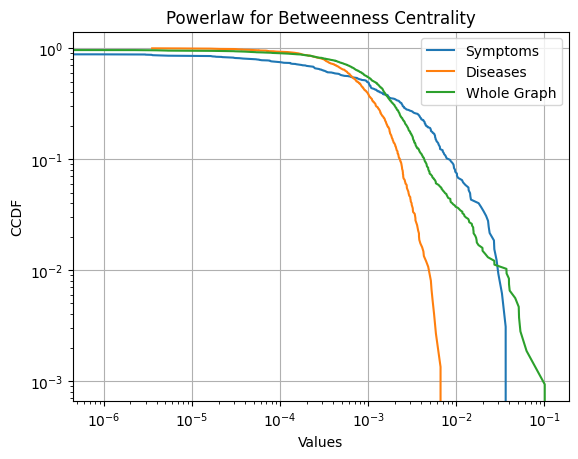
\includegraphics[width=1\columnwidth]{bet_all.png}
    \caption{Betweenness Centrality CDFs}
    \label{fig:bet_all}
 \end{figure}

Upon dissecting the centrality values into symptoms and diseases (see Figures~\ref{fig:bet_diseases} and~\ref{fig:bet_symptoms}), 
a notable observation emerges: symptoms tend to have higher betweenness centrality compared to diseases. To decipher the 
significance of this result, it's essential to delve into the interpretation of betweenness centrality.

\begin{figure}[H]
    \centering
    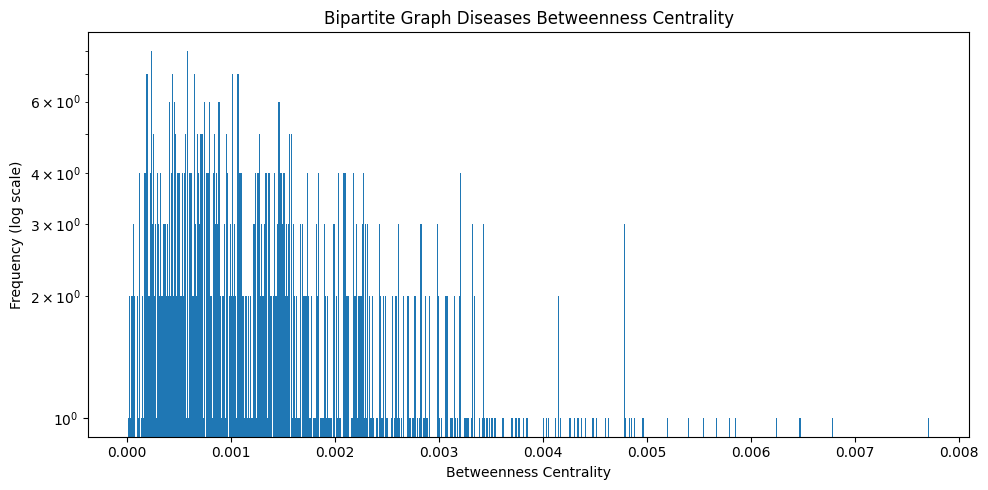
\includegraphics[width=1\columnwidth]{bet_diseases.png}
    \caption{Betweenness Centrality of the diseases}
    \label{fig:bet_diseases}
\end{figure}

\begin{figure}[H]
    \centering
    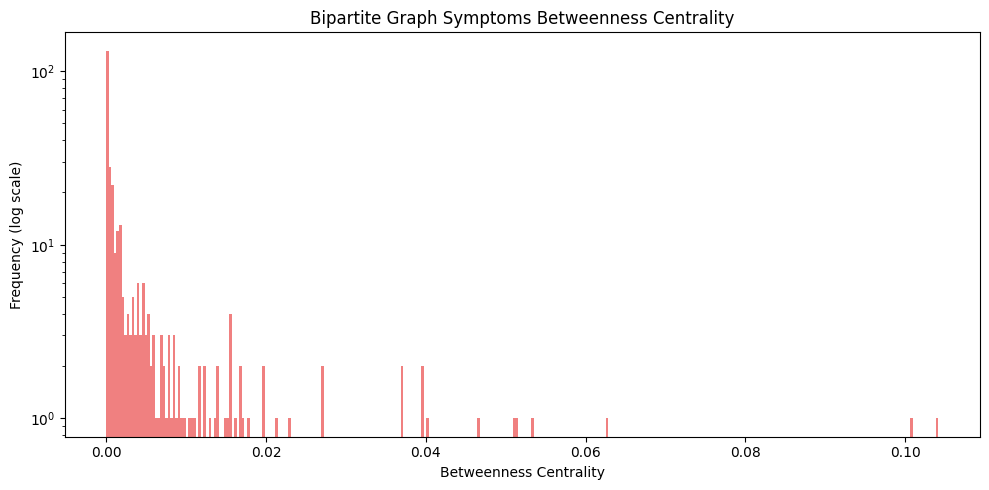
\includegraphics[width=1\columnwidth]{bet_symptoms.png}
    \caption{Betweenness Centrality of the symptoms}
    \label{fig:bet_symptoms}
\end{figure}

In general, a symptom exhibits high betweenness centrality when it is linked to numerous diseases, and these diseases, 
in turn, are connected to a relatively limited set of symptoms. Conversely, a disease attains high betweenness centrality 
when it connects to numerous symptoms, and these symptoms are associated with relatively few diseases.

Analyzing our results (L1 and L2), it becomes evident that the higher betweenness centrality of symptoms is attributed 
to their connections with a multitude of diseases, while diseases, on the contrary, are linked to a relatively limited 
number of symptoms. From a predictive standpoint, this outcome presents a challenge as each symptom is not sufficiently 
specific, contributing to a broad array of disease classes.

Figure~\ref{fig:bet_top} highlights the top 10 nodes with the highest betweenness centrality, all of which are symptoms. 
As anticipated, these symptoms are more generic in nature, aligning with their central role in connecting various diseases.

\begin{figure}[H]
    \centering
    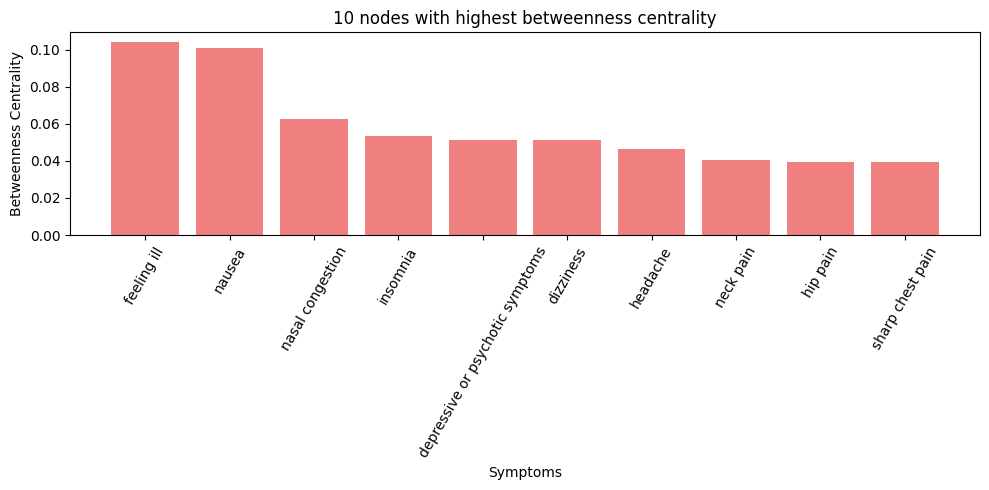
\includegraphics[width=1\columnwidth]{bet_top.png}
    \caption{Top 10 nodes with the highest betweenness centrality}
    \label{fig:bet_top}
\end{figure}

% END: betweenness centrality

\subsection{Communities}

% BEGIN: communities
The identification of communities within the network serves a dual purpose – facilitating network interpretation 
and enhancing the capabilities of our ML prediction model.

From a network interpretation perspective, communities offer insights into disease-symptom relationships. 
A community of symptoms signifies a set of symptoms that frequently co-occur within the same diseases, while a 
community of diseases identifies a set of diseases often co-occurring within the same symptoms. The sizes of 
different communities are illustrated in Figure~\ref{fig:com_sizes_all}.

\begin{figure}[H]
    \centering
    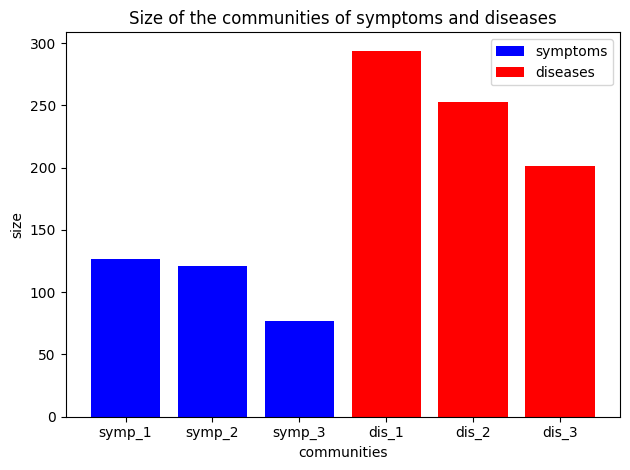
\includegraphics[width=1\columnwidth]{com_sizes_all.png}
    \caption{Sizes of the communities of symptoms and diseases}
    \label{fig:com_sizes_all}
\end{figure}

For clinical relevance, examining symptoms communities provides valuable information about diseases associated 
with these symptoms. This is exemplified in Figures~\ref{fig:com1_symptoms}, \ref{fig:com2_symptoms}, 
and \ref{fig:com3_symptoms}. As an illustration, in the community 1 of symptoms (Figure~\ref{fig:com1_symptoms}), 
'herniated disk' is the third most pointed disease by the symptoms of the community, with each symptom pointing, 
on average, to three diseases.

\begin{figure}[H]
    \centering
    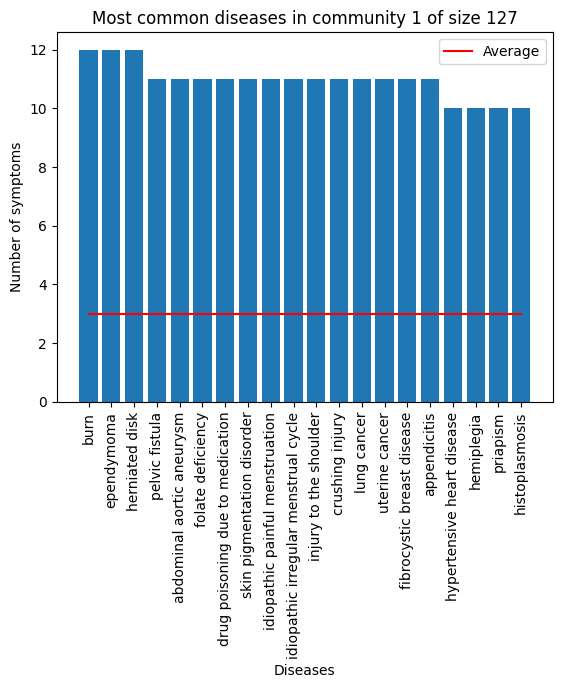
\includegraphics[width=1\columnwidth]{com1_symptoms.png}
    \caption{Community 1 of symptoms}
    \label{fig:com1_symptoms}
\end{figure}

A similar study can be conducted for communities of diseases, as depicted in Figures~\ref{fig:com1_diseases}, 
\ref{fig:com2_diseases}, and \ref{fig:com3_diseases}. This information aids in profiling diseases and understanding 
the significance of each symptom. For instance, in community 1 of diseases (Figure~\ref{fig:com1_diseases}), 
the symptom 'sharp abdominal pain' is present in almost half of the diseases in the community, indicating its 
generic nature and limited discriminatory value.

\begin{figure}[H]
    \centering
    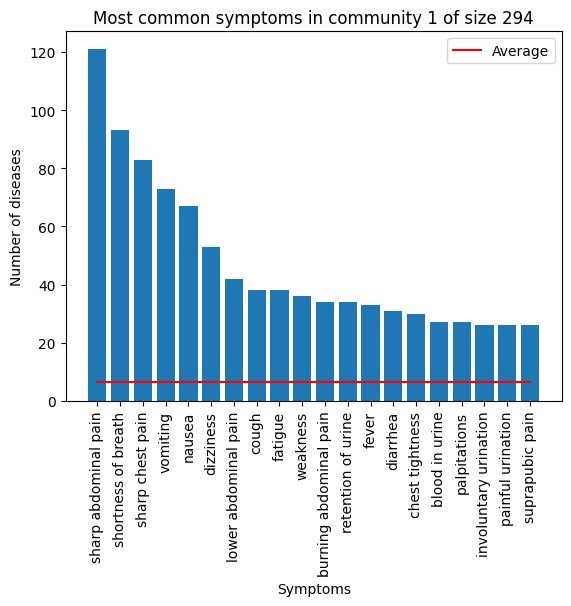
\includegraphics[width=1\columnwidth]{com1_diseases.png}
    \caption{Community 1 of diseases}
    \label{fig:com1_diseases}
\end{figure}

Transitioning to the creation of features for the ML model, two types of features were developed:\\

\begin{itemize}
    \setlength\itemsep{1em} % set space between items

    \item \textbf{Community Count:} This feature counts how many symptoms of the symptom vector belong to each community. 
    Each symptom community is characterized by different pointed diseases. The model can learn to prioritize 
    diseases associated with the community with the highest count.
    
    \item \textbf{Community Size:} This feature replaces each symptom in the symptom vector with the size of the 
    community to which the symptom belongs. It enables the model to distinguish between symptoms belonging to small and 
    large communities, injecting community information into the model beyond basic one-hot encoding of symptoms.
\end{itemize}

\vspace{0.4cm}
It is noteworthy that communities can also contribute to improving the computational efficiency of the model. 
For example, a symptom associated with many diseases may be less informative and could potentially be removed from the 
symptom vector. However, we opted for a comprehensive approach using a combination of L1 and L2 measures to address this issue.

% END: communities

\subsection{Most Important Actors}
% BEGIN: most important symptoms/diseases (4 classes)

As anticipated our goal is not only to extract features from the network but also to exploit this latter to improve the 
computational efficiency of the model. The idea is to reduce the number of symptoms, retaining only the most important
ones, to reduce the training time, while maintaining an as high as possible accuracy. To this end, we tested different
approaches, involving betweenness centrality or even the degree of the unipartite projection of symptoms.


% END: most important symptoms/diseases (4 classes)



% ------------- Appendix Figures -------------
% Figures to be placed in the appendix

\begin{figure}[H]
    \centering
    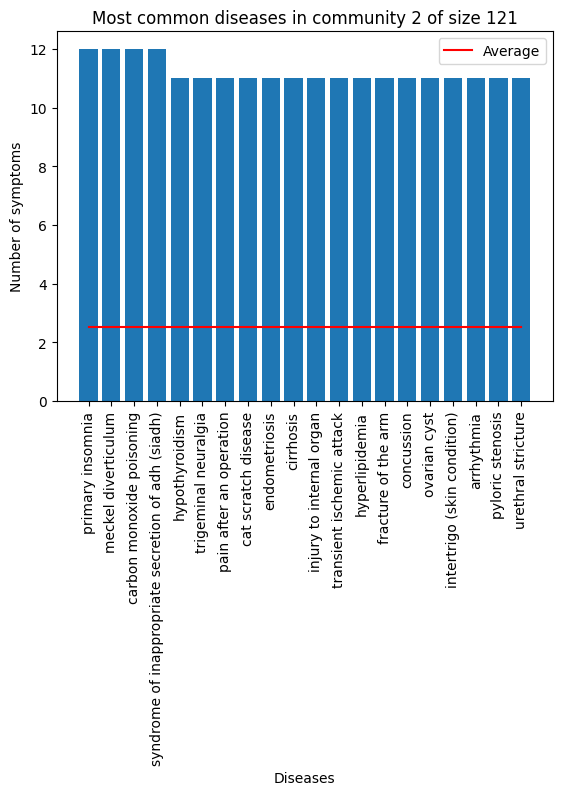
\includegraphics[width=1\columnwidth]{com2_symptoms.png}
    \caption{Community 2 of symptoms}
    \label{fig:com2_symptoms}
\end{figure}

\begin{figure}[H]
    \centering
    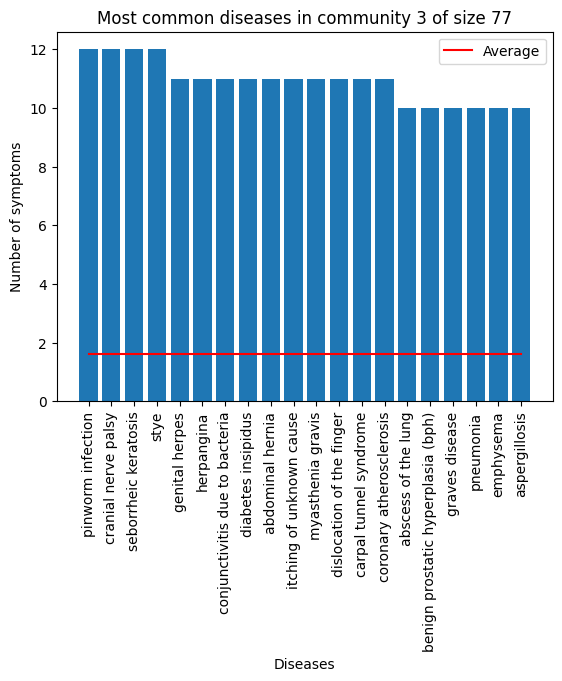
\includegraphics[width=1\columnwidth]{com3_symptoms.png}
    \caption{Community 3 of symptoms}
    \label{fig:com3_symptoms}
\end{figure}



\begin{figure}[H]
    \centering
    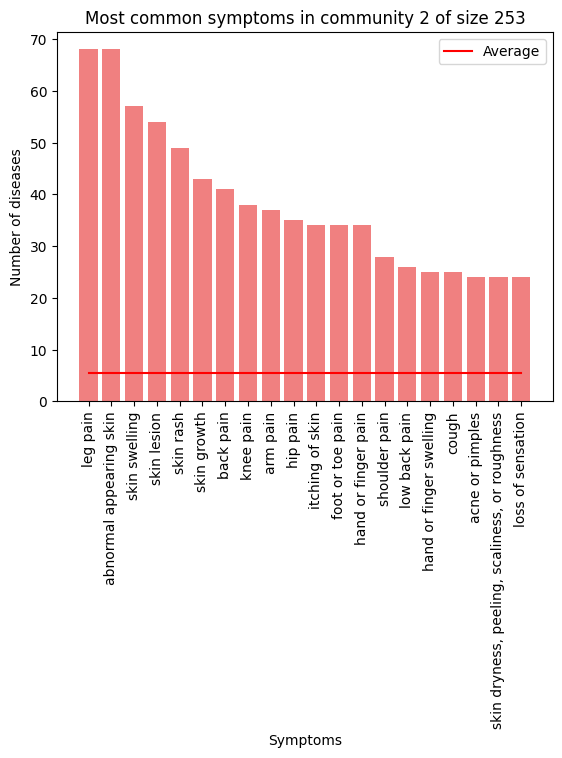
\includegraphics[width=1\columnwidth]{com2_diseases.png}
    \caption{Community 2 of diseases}
    \label{fig:com2_diseases}
\end{figure}

\begin{figure}[H]
    \centering
    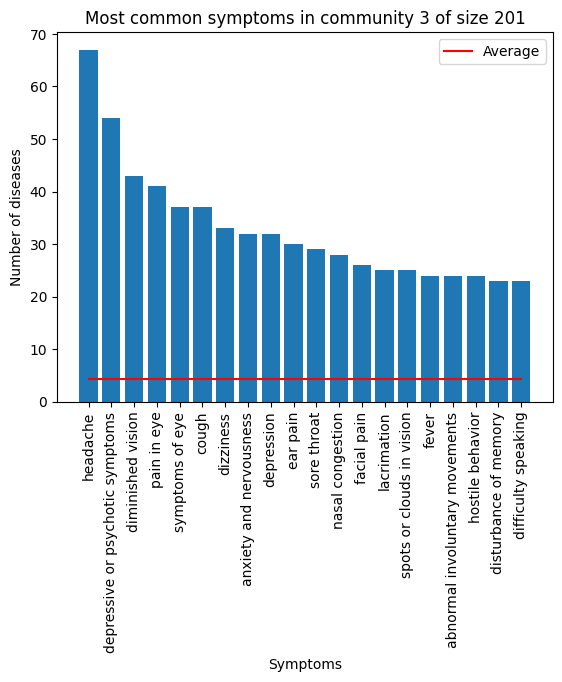
\includegraphics[width=1\columnwidth]{com3_diseases.png}
    \caption{Community 3 of diseases}
    \label{fig:com3_diseases}
\end{figure}